\begin{dang}{Tìm các khoảng đơn điệu (khảo sát chiều biến thiên)}
 \baitoan Tìm các khoảng đơn điệu (khảo sát chiều biến thiên) của hàm số $y=f(x)$.\\
 \phuongphap
 \begin{itemize}
 \item \textbf{Bước 1.} Tìm tập xác định $\mathscr{D}$ của hàm số. Tính đạo hàm $y'=f'(x)$.
 \item \textbf{Bước 2.} Tìm các điểm tại đó $f'(x)=0$ hoặc $f'(x)$ không xác định.
 \item \textbf{Bước 3.} Sắp xếp các điểm theo thứ tự tăng dần và lập bảng biến thiên (xét dấu $y'$).
 \item \textbf{Bước 4.} Từ bảng biến thiên, kết luận: $y'>0 \Rightarrow $ đồng biến và $y'<0 \Rightarrow $ nghịch biến.
 \end{itemize}
\end{dang}
%\begin{vd}%[2D1Y1-1]
% Tìm khoảng đơn điệu của các hàm số sau
% \begin{listEX}[3]
% \item $y=x^2-4x$.
% \item $y=-x^2+5x-4$.
% \item $y=x^3-3x^2+1$.
% \item $y=-x^3+3x^2+9x$.
% \item $y=\dfrac{x+1}{x-1}$.
% \item $y=\dfrac{3-x}{x+1}$.
% \item $y=\dfrac{x^2-3x}{x+1}$.
% \item $y=\dfrac{x^2+x+4}{x+1}$
% \item $y=\sqrt{9-x^2}$.
% \end{listEX}
% \loigiai{}
%\end{vd}
\begin{vd}%[2D1Y1-1]
 Tìm khoảng đơn điệu của các hàm số sau
 \begin{listEX}[3]
 \item $y=x^3-3x^2+1$.
 \item $y=-x^3+3x^2+9x$.
 \item $y=x^3+2$.
 \item $y=\dfrac{x+1}{x-1}$.
 \item $y=\dfrac{3-x}{x+1}$.
 \item $y=\dfrac{x^2-3x}{x+1}$.
 \item $y=\dfrac{x^2+x+4}{x+1}$.
 \item $y=\sqrt{9-x^2}$.
 \item $y=x^3+5x-\cos x$
 \end{listEX}
 \loigiai{}
\end{vd}
\begin{vd}
 Tìm các khoảng đơn điệu của hàm số $y=f(x)$ có đồ thị hoặc bảng biến thiên như hình vẽ
 \begin{listEX}[3]
 \item
 \begin{tikzpicture}[>=stealth,x=1cm,y=1cm,scale=0.7,font=\footnotesize]
 \path
 (0,0) coordinate (O)
 (-0.5,0) coordinate (A)
 %	Các điểm mút cho lệnh controls:
 (-1.4,1) coordinate (N)
 (0,2) coordinate (D)
 (0.68,0.95) coordinate (M1)
 (1.4,-0.6) coordinate (Q)
 (2.1,2.6) coordinate (M2)
 ;
 %Vẽ đường cong:
 %	\draw[red] (N)--(D)--(Q)--(M2);
 \draw[thick,red,smooth] (N)..controls +(40:0.25) and +(-175:0.5)..(D)..controls +(-15:0.5) and +(170:0.25)..(Q)..controls +(10:0.25) and +(-100:0.25)..(M2);
 %Vẽ hệ trục tọa dộ:
 \draw[->] (-2,0)--(0,0) node[below left]{$O$}--(2.5,0) node[below]{$x$};
 \draw[->] (0,-1) --(0,3) node[left]{$y$};
 %	Vẽ nét đứt+node:
 \foreach \p/\n/\r in {N/-2/-90,M1/1/-90,Q/2/90,M2/3/-90}
 \draw[dashed](\p)--($(A)!(\p)!(O)$)node[shift={(\r:3mm)}]{$ \n $} ;
 \path ($(A)!(N)!(O)$)coordinate (A1) ($(A)!(M1)!(O)$)coordinate (B1)($(A)!(M2)!(O)$)coordinate (B3) ($(A)!(Q)!(O)$)coordinate (B2);
 \foreach \p/\r in {M1,M2,Q,D,A1,B1,B2,B3,N}
 \fill (\p) circle (1pt) ;
 \end{tikzpicture}
 \item*[d)]
 
\begin{tikzpicture}
 \tkzTabInit[lgt=1.2,espcl=2,deltacl=0.6]
 {$x$ /0.6,$y'$ /0.6,$y$ /1.8}
 {$-\infty$,$-4$,$1$,$2$,$+\infty$}
 \tkzTabLine{,+,$0$,-,$0$,+,$0$,-,}
 \tkzTabVar{-/$-\infty$, +/$5$,-/$-1$,+/$3$,-/$-\infty$}
 \end{tikzpicture}
 \item
 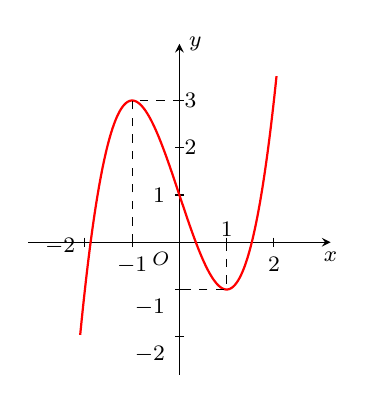
\begin{tikzpicture}[>=stealth,scale=0.6,font=\footnotesize]
 \def\a{1} % Hệ số a phải khác 0
 \def\b{0}
 \def\c{-3}
 \def\d{1}
 \def\xmin{-3}\def\xmax{3}\def\ymin{-2}\def\ymax{4}
 \draw[->] (\xmin-0.2,0)--(\xmax+0.2,0) node[below] {$x$};
 \draw[->] (0,\ymin-0.8)--(0,\ymax+0.2) node[right] {$y$};
 \foreach \x in {-1,2}\draw (\x,0.1)--(\x,-0.1) node [below] {\footnotesize $\x$};
 \foreach \x in {1}\draw (\x,0.1)--(\x,-0.1) node [above=0.1] {\footnotesize $\x$};
 \foreach \x in {-2}\draw (\x,0.1)--(\x,-0.1) node [left] {$\x$};
 \foreach \y in {1}\draw (0.1,\y)--(-0.1,\y) node [left] {\footnotesize $\y$};
 \foreach \y in {2,3}\draw (0.1,\y)--(-0.1,\y) node [right=0.1] {\footnotesize $\y$};
 \foreach \y in {-1,-2}\draw (0.1,\y)--(-0.1,\y) node [below left] {\footnotesize $\y$};
 \draw (0,0) node[below left]{\scriptsize $O$};
 \clip (-2.5,-2.3)rectangle(3.5,3.5);
 \draw[samples=200,smooth,thick,red,,domain=-2.1:2.3]plot(\x,{\a*(\x)^3+(\b)*(\x)^2+(\c)*\x+(\d)});
 \draw[dashed] (-1,0)--(-1,3)--(0,3);
 \draw[dashed] (1,0)--(1,-1)--(0,-1);
 \end{tikzpicture}
 \item*[e)]
 \begin{tikzpicture}
 \tkzTabInit[lgt=1.2,espcl=2,deltacl=0.6]
 {$x$ /0.6,$y'$ /0.6,$y$ /1.8}
 {$-\infty$,$-1$,$2$,$5$,$+\infty$}
 \tkzTabLine{,-,$0$,+,d,-,$0$,-,}
 \draw (N12)node[below](A){$+\infty$} (N23) node[above](B){$-1$} (N32)[below]node(C){$3$} ($(N32)!0.5!(N53)+(0,0.2)$)node(D){$1$} (N53)node[above](E){$-\infty$};
 \foreach \x/\y in {A/B,B/C,C/D,D/E}
 {\draw[-stealth] (\x)--(\y);}
 \end{tikzpicture}
 \item
	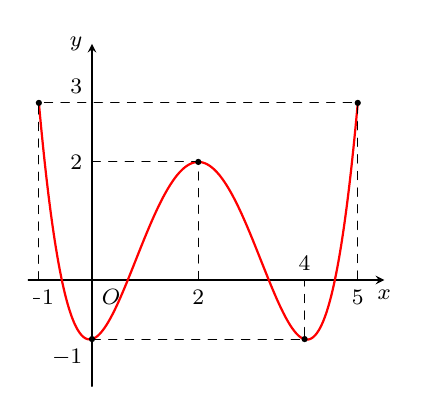
\begin{tikzpicture}[scale=0.75, font=\footnotesize, line join=round, line cap=round, >=stealth,x=.9cm]
 \def\xt{-1.2} \def\xp{5.5} \def\yt{4} \def\yd{-1.8}
 \draw[->] (\xt,0)--(\xp,0) node [below]{$x$};
 \draw[->] (0,\yd)--(0,\yt) node [left]{$y$};
 \node at (0,0) [below right]{$O$};
 \clip (\xt+0.1,\yd) rectangle (\xp-0.1,\yt-0.1);
 \draw[smooth,samples=300,thick,red,domain=-1:5] plot(\x,{31/180*(\x)^4-62/45*(\x)^3+97/36*(\x)^2+11/45*(\x)-1});
 \draw[dashed] (-1,0) node [below]{$-1$} -- (-1,3) -- (0,3) node [above left]{$3$} -- (5,3) -- (5,0) node [below]{$5$};
 \draw[dashed] (0,2) node [left]{$2$} -- (2,2) -- (2,0) node [below]{$2$};
 \draw[dashed] (0,-1) node [below left]{$-1$} -- (4,-1) -- (4,0) node [above]{$4$};
 \foreach \x/\y in {-1/3,0/-1,2/2,4/-1,5/3}
 \fill (\x,\y) circle (1.5pt);
% \node at (2,-2.2){\text{a)}};
\end{tikzpicture}
 \item*[f)]
 
\begin{tikzpicture}
 \tkzTabInit[lgt=1.2,espcl=2.65,deltacl=0.6]
 {$x$ /0.6,$y'$ /0.6,$y$ /1.8}
 {$-\infty$,$1$,$2$,$+\infty$}
 \tkzTabLine{,+,d,+,d,-,}
 \tkzTabVar{-/$-\infty$, +D-/$+\infty$/$-\infty$,+/$3$,-/$-\infty$}
 \end{tikzpicture}
 \end{listEX}
 \loigiai{}
\end{vd}
\begin{vd}%[2D1Y1-1]
 Tìm các khoảng đơn điệu của hàm số $y=f(x)$, biết
 \begin{listEX}[2]
 \item $f'(x)=x(3x-4)^2(x+2)^3$, $\forall x \in \mathbb{R}$.
 \item $f'(x)=x^2(3x+4)^5(3-x)^4, \forall x\in \mathbb{R}$.
 \item
 $y=f(x)$ xác định trên $\mathbb{R}\setminus \{2\}$ và có bảng xét dấu đạo hàm như sau\\
 \centering 
\begin{tikzpicture}
 \tkzTabInit[lgt=.9,espcl=1.2,deltacl=0.6]
 {$x$ /0.6,$y'$ /0.6}
 {$-\infty$,$-1$,$2$,$3$,$+\infty$}
 \tkzTabLine{,-,$0$,+,d,+,$0$,+,}
 \end{tikzpicture}
 \item
 $y=f(x)$ xác định trên $\mathbb{R}$ và có bảng xét dấu đạo hàm như sau\\
 \centering
 
\begin{tikzpicture}
 \tkzTabInit
 [nocadre=false,lgt=.9,espcl=1.2,deltacl=0.6]
 {$x$/0.6, $y'$/0.6}
 {$-\infty$,$-2 $,$0 $,$2$,$+\infty$}
 \tkzTabLine{, - , d , - , 0 , + , 0, - , }
 \end{tikzpicture}
\item $y=f(x)$ xác định trên $\mathbb{R}$ và có đồ thị của $y=f'(x)$ như hình vẽ\\
\centering
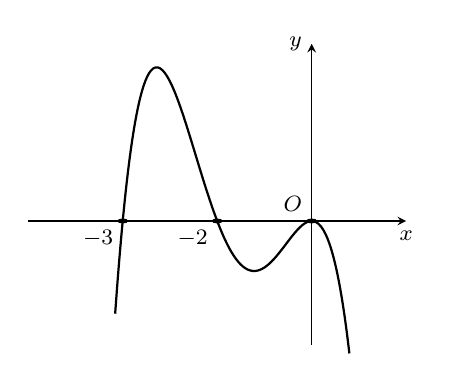
\begin{tikzpicture}[>=stealth,font=\footnotesize, xscale=1.2, yscale=0.45]
 \draw[->] (-3,0) -- (1,0) node[below] {$x$};
 \draw[->] (0,-3.5) -- (0,5) node[left] {$y$};
 \filldraw (0,0) node[above left=-0.1] {$O$} circle (1.5pt);
 \draw[thick,smooth,samples=100,domain=-2.08:0.4] plot(\x,{-7*(\x)^2*(\x+1)*(\x+2)});
 \filldraw (-2,0) node[below left=-0.1] {$-3$} circle (1.5pt);
 \filldraw (-1,0) node[below left=-0.1] {$-2$} circle (1.5pt);
\end{tikzpicture}
\item $y=f(x)$ xác định trên $\mathbb{R}$ và có đồ thị của $y=f'(x)$ như hình vẽ\\
\centering
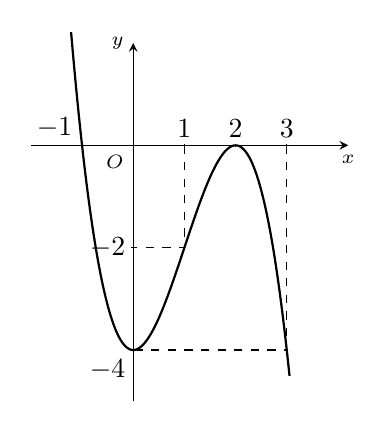
\begin{tikzpicture}[>=stealth,x=1cm,y=1cm,scale=0.65]
 \def\a{-1} % Hệ số a phải khác 0
 \def\b{3}
 \def\c{0}
 \def\d{-4}
 \draw[->] (-2,0) -- (4.2,0)node[below]{\scriptsize $x$};
 \draw[->] (0,-5) -- (0,2) node[left] {\scriptsize $y$};
 \draw (0,0)node[below left]{\scriptsize $O$};
 \draw[thin] (-1,1pt)--(-1,-1pt) node [above left] {$-1$} (1,1pt)--(1,-1pt) node [above] {$1$} (2,1pt)--(2,-1pt) node [above] {$2$} (3,1pt)--(3,-1pt) node [above] {$3$} (-1pt,-2)--(1pt,-2) node [left] {$-2$} (-1pt,-4)--(1pt,-4) node [below left] {$-4$} ;
 \draw[dashed] (1,0)--(1,-2)--(0,-2) (3,0)--(3,-4)--(0,-4);
 \clip (-2,-4.5)rectangle(4,2.2);
 \draw[thick,samples=150,smooth,domain=-1.25:5] plot(\x,{\a*(\x)^3+(\b)*(\x)^2+(\c)*\x+(\d)});
\end{tikzpicture}
 \end{listEX}
 \loigiai{}
\end{vd}
\begin{vd}
 \immini{
 Máng trượt của một cầu trượt cho trẻ em (\textit{Hình 5a}) được uốn từ một tấm kim loại có bề rộng $80$ cm, mặt cắt được mô tả ở \textit{Hình 5b}. Nhà thiết kế khuyến cáo, diện tích mặt cắt càng lớn thì càng đảm bảo an toàn cho trẻ em.
 }{
 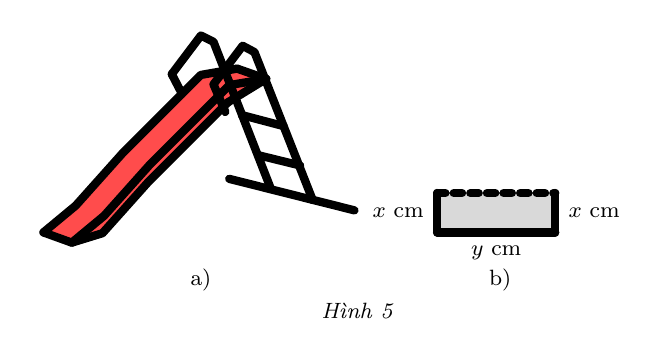
\begin{tikzpicture}[scale=1, font=\footnotesize, line join=round, line cap=round, >=stealth,line width=3.pt]
 \clip(-0.2,-1.2) rectangle (7.5,2.6);
 \fill[line width=3.pt,color=red,fill=red,fill opacity=0.7] (0,0)--(0.41,0.34)--(1,1)--(1.76,1.76)--(2,2)--(2.46,2.08)--(2.83,1.95)--(2.34,1.65)--(1.34,0.65)--(0.75,-0.01)--(0.36,-0.13)-- cycle;
 \draw (0,0)--(0.41,0.34)--(1,1)--(2,2)--(2.46,2.08);
 \draw (0,0)--(0.36,-0.13)--(0.77,0.21)--(0.77,0.21)--(1.36,0.87)--(2.36,1.87)--(2.83,1.95);
 \draw (0.36,-0.13)--(0.75,-0.01)--(1.34,0.65)--(2.34,1.65);
 \draw (2.36,0.68)-- (3.95,0.28);
 \draw (3.42,0.41)--(2.68,2.29)--(2.53,2.37)--(2.16,1.88)--(2.31,1.53);
 \draw (1.63,2.01)--(2,2.5)-- (2.16,2.42)--(2.89,0.55);
 \draw (1.63,2.01)--(1.76,1.76) (2.73,0.98)--(3.26,0.85) (2.52,1.49)--(3.05,1.35);
 \draw (2.34,1.65)--(2.83,1.95)--(2.46,2.08);
 \draw (2,-0.6)node{a)};
 \fill[line width=3.pt,fill=gray,fill opacity=0.3] (5,0.5)--(5,0)--(6.5,0)--(6.5,0.5)--cycle;
 \draw (5,0.5)--(5,0) node [left ,sloped,pos=0.5,rotate=90] {$x$ cm};
 \draw (5,0)--(6.5,0) node [below,sloped,pos=0.5] {$y$ cm};
 \draw (6.5,0)--(6.5,0.5) node [right,sloped,pos=0.5,rotate=-90] {$x$ cm};
 \draw[dashed] (5,0.5)--(6.5,0.5);
 \draw (5.8,-0.6)node{b)};
 \draw (4,-1)node{\textit{Hình 5}};
 \end{tikzpicture}
 }
 \begin{enumerate}
 \item Gọi $S$ là diện tích mặt cắt. Tìm điều kiện của $x$ và viết công thức tính $S$ theo $x$.
 \item Với $x$ đạt giá trị bằng bao nhiêu thì cầu trượt đảm bảo an toàn nhất cho trẻ em?
 \end{enumerate}
 \loigiai{
 \begin{enumerate}
 \item Do tấm kim loại có bề rộng $80 \mathrm{~cm}$ nên ta có: $2x+y=80 \Leftrightarrow y=80-2x$.\\
 Để có thể thiết kế được máng trượt thì $y>0 \Leftrightarrow 80-2 x>0 \Leftrightarrow x<40$. Suy ra $0<x<40$.\\
 Diện tích của mặt cắt máng trượt là: $S=x y=x(80-2x)=-2x^2+80x$.
 \item Ta có:
 \allowdisplaybreaks
 \begin{eqnarray*}
 S(x)&=&-2x^2+80x \text{ với } x\in(0; 40);\\
 S'(x)&=&-4 x+80 \\
 S'(x)&=&0 \Leftrightarrow-4 x+80=0 \Leftrightarrow x=20.
 \end{eqnarray*}
 Bảng biến thiên của hàm số $S(x)$ như sau:
 \begin{center}
 
\begin{tikzpicture}[font=\footnotesize,thick,>=stealth]
 \tikzset{double style/.append style={double distance=1.5pt}}
 \tkzTabInit[nocadre=false,lgt=1.2,espcl=2.5,deltacl=0.6,lw=.75pt,color,colorL=green!50,colorV=green!50]
 {$x$ /0.7, $S'(x)$ /0.8, $S(x)$ /2}
 {$0$,$20$,$40$}
 \tkzTabLine{ ,+,,-, }
 \tkzTabVar{-/$0$,+/$800$,-/$0$}
 \end{tikzpicture}
 \end{center}
 Do đó, hàm số $S(x)$ đạt cực đại tại $x=20$ và $S_{\text{CĐ}}=800$.\\
 Vậy để cầu trượt đảm bảo an toàn nhất cho trẻ em thì $x=20$ (cm).
 \end{enumerate}
 }
\end{vd}
\BTTN
\Opensolutionfile{ans}[ans/2D1-1-DANG-1]
\begin{ex}%[2D1B1-1]
 Cho hàm số $y=x^3 -3x^2$. Mệnh đề nào sau đây đúng?
 \choice
 {\True Hàm số nghịch biến trên khoảng $(0;2)$}
 {Hàm số nghịch biến trên khoảng $(2;+ \infty)$}
 {Hàm số đồng biến trên $(0;2)$}
 {Hàm số nghịch biến trên $(-\infty; 0)$}
 \loigiai{
 \begin{itemize}
 \item $\mathscr D = \mathbb{R}$.
 \item $y'= 3x^2 -6x=0 \Leftrightarrow x=0; x=2$.
 \item Bảng biến thiên
 \begin{center}
 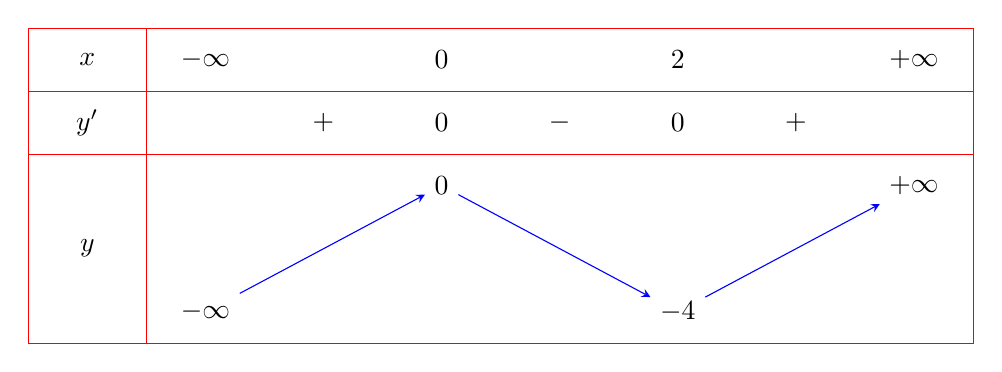
\begin{tikzpicture}[yscale=.8,xscale=1.5,]
 \begin{scope}[shift={(-.5,.5)}]
 \draw[red]
 (0,0) rectangle +(8,-5)
 (0,-1)--+(0:8) (0,-2)--+(0:8) (1,0)--+(-90:5);
 \end{scope}
 \path
 (0,0) node{$x$} % <<< dòng 1
 ++(0:1) node{$-\infty$}
 ++(0:2) node{$0$}
 ++(0:2) node{$2$}
 ++(0:2) node{$+\infty$}
 (0,-1) node{$y'$} % <<< dòng 2
 ++(0:2) node{$+$}
 ++(0:1) node{$0$}
 ++(0:1) node{$-$}
 ++(0:1) node{$0$}
 ++(0:1) node{$+$}
 (0,-3) node{$y$} % <<< dòng 3
 ++(0:1) ++(-90:1) node (A) {$-\infty$}
 ++(0:2) ++(+90:2) node (B) {$0$}
 ++(0:2) ++(-90:2) node (C) {$-4$}
 ++(0:2) ++(+90:2) node (D) {$+\infty$};
 \draw[-stealth,blue] (A)--(B);
 \draw[-stealth,blue] (B)--(C);
 \draw[-stealth,blue] (C)--(D);
 \end{tikzpicture}
 \end{center}
 \end{itemize}
 Dựa vào bảng biến thiên ta thấy hàm số nghịch biến trên khoảng $(0;2)$.}
\end{ex}
\begin{ex}%[2D1B1-1]
 Hàm số $y=- \dfrac{1}{3} x^3 - \dfrac{1}{2} x^2 -2$ nghịch biến trên khoảng nào dưới đây?
 \choice
 {$\mathbb{R} $}
 {$(- \infty; 1) $}
 {$ (-1;0)$}
 {\True $(-\infty;-1) $}
 \loigiai{
 \begin{itemize}
 \item $\mathscr D = \mathbb{R}$.
 \item $y'= -x^2-x=0 \Leftrightarrow x=-1; x=0$.
 \item Bảng biến thiên
 \begin{center}
 \begin{tikzpicture}[yscale=.8,xscale=1.5,]
 \begin{scope}[shift={(-.5,.5)}]
 \draw[red]
 (0,0) rectangle +(8,-5.1)
 (0,-1)--+(0:8) (0,-2)--+(0:8) (1,0)--+(-90:5);
 \end{scope}
 \path
 (0,0) node{$x$} % <<< dòng 1
 ++(0:1) node{$-\infty$}
 ++(0:2) node{$-1$}
 ++(0:2) node{$0$}
 ++(0:2) node{$+\infty$}
 (0,-1) node{$y'$} % <<< dòng 2
 ++(0:2) node{$-$}
 ++(0:1) node{$0$}
 ++(0:1) node{$+$}
 ++(0:1) node{$0$}
 ++(0:1) node{$-$}
 (0,-3) node{$y$} % <<< dòng 3
 ++(0:1) ++(90:1) node (A) {$+\infty$}
 ++(0:2) ++(-90:2) node (B) {$-\dfrac{13}{6}$}
 ++(0:2) ++(90:2) node (C) {$-2$}
 ++(0:2) ++(-90:2) node (D) {$-\infty$};
 \draw[-stealth,blue] (A)--(B);
 \draw[-stealth,blue] (B)--(C);
 \draw[-stealth,blue] (C)--(D);
 \end{tikzpicture}
 \end{center}
 \end{itemize}
 Dựa vào bảng biến thiên ta thấy hàm số đã cho nghịch biến trên khoảng $(-\infty; -1 )$.}
\end{ex}
\begin{ex}%[2D1B1-1]
 Cho hàm số $y= x^3 + 3x -4 $. Mệnh đề nào dưới đây đúng?
 \choice
 {Hàm số đồng biến trên $(-1;1)$}
 {Hàm số nghịch biến trên $\mathbb{R}$}
 {Hàm số đồng biến trên $(-\infty; -1)$ và trên $(-1; +\infty)$}
 {\True Hàm số đồng biến trên $\mathbb{R}$}
 \loigiai{
 \begin{itemize}
 \item $\mathscr D = \mathbb{R}$.
 \item $y'= 3x^2 + 3 \Rightarrow y'>0, \forall x \in \mathscr D $.
 \end{itemize}
 Suy ra hàm số đã cho đồng biến trên $\mathbb{R}$.}
\end{ex}
\begin{ex}%[2D1B1-1]
 Cho hàm số $y= x^4 + 8x^2 -4 $. Mệnh đề nào dưới đây \textbf{sai}?
 \choice
 {\True Hàm số đồng biến trên $(-\infty; -2)$ và $(2;+\infty)$}
 {Hàm số đồng biến trên $(0;+\infty) $}
 {Hàm số nghịch biến trên $(- \infty; 0) $}
 {Hàm số nghịch biến trên $(-\infty; -2) $ và $(-1; 0)$}
 \loigiai{
 \begin{itemize}
 \item $\mathscr D = \mathbb{R}$
 \item 	$y'= 4x^3 + 16x =0 \Leftrightarrow x=0$.
 \item Bảng biến thiên
 \begin{center}
 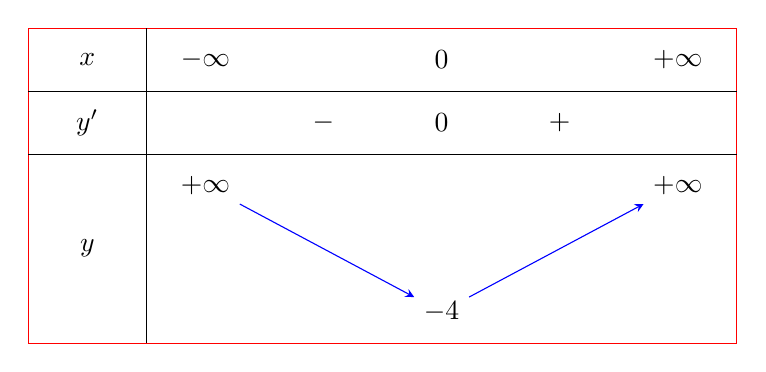
\begin{tikzpicture}[yscale=.8,xscale=1.5,]
 \begin{scope}[shift={(-.5,.5)}]
 \draw[red] (0,0) rectangle +(6,-5);
 \draw (0,-1)--+(0:6) (0,-2)--+(0:6) (1,0)--+(-90:5);
 \end{scope}
 \path
 (0,0) node{$x$} % <<< dòng 1
 ++(0:1) node{$-\infty$}
 ++(0:2) node{$0$}
 ++(0:2) node{$+\infty$}
 (0,-1) node{$y'$} % <<< dòng 2
 ++(0:2) node{$-$}
 ++(0:1) node{$0$}
 ++(0:1) node{$+$}
 (0,-3) node{$y$} % <<< dòng 3
 ++(0:1) ++(90:1) node (A) {$+\infty$}
 ++(0:2) ++(-90:2) node (B) {$-4$}
 ++(0:2) ++(90:2) node (C) {$+\infty$};
 \draw[-stealth,blue] (A)--(B);
 \draw[-stealth,blue] (B)--(C);
 \end{tikzpicture}
 \end{center}
 \end{itemize}
 Dựa vào bảng biến thiên ta thấy trên khoảng $(-\infty; -2)$ hàm số nghịch biến.
 }
\end{ex}
\begin{ex}%[2D1B1-1]
 Khoảng nghịch biến của hàm số $ y=-2x^4-x^2-1 $ là khoảng nào dưới đây ?
 \choice
 {$\left(-\dfrac{1}{2} ;+\infty\right)$}
 {$(-\infty ; 0)$}
 {$(-\infty ;+\infty)$}
 {\True$(0 ;+\infty)$}
 \loigiai{
 \begin{itemize}
 \item $\mathscr{D} = \mathbb{R}$.
 \item 	$ y'=-8x^3-2x =0\Leftrightarrow x=0 $.
 \item Bảng biến thiên:
 \begin{center}
 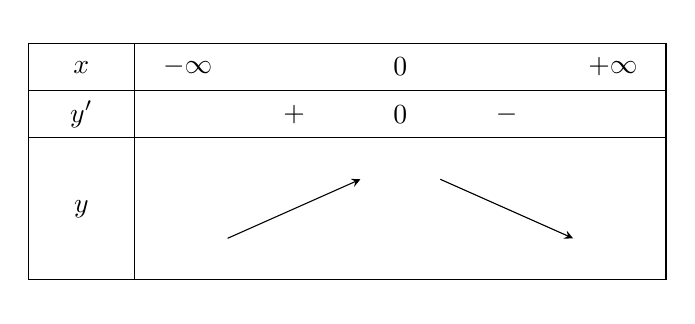
\begin{tikzpicture}[yscale=0.6,xscale=1.35]
 \def\c{5}%số cột
 \def\d{4}%số dòng
 \foreach \x in {0,...,\c}{
 \foreach \y in {0,...,\d}
 \path[yscale=-1] (\x,\y) node[gray!0,minimum size=1cm] (\x\y) {\x\y};
 }
 \draw[shift={(-0.5,0.5)}]
 (0,0) rectangle (\c+1,-\d-1)
 (0,-1)--(\c+1,-1)
 (0,-2)--(\c+1,-2)
 (1,0)--(1,-\d-1);
 \path
 (00) node {$x$}(10) node {$-\infty$}(30) node {$0$}(50) node {$+\infty$}
 (01) node {$y'$}(21) node {$+$}(31) node {$0$}(41) node {$-$}
 (03) node {$y$}
 ;
 \foreach \a/\b in {14/32,32/54}
 \draw[->,>=stealth] (\a)--(\b);
 \end{tikzpicture}
 \end{center}
 \end{itemize}
 Dựa vào bảng biến thiên, hàm số nghịch biến trên khoảng $(0 ;+\infty)$.
 }
\end{ex}
\begin{ex}%[2D1Y1-1]
 Cho hàm số $ y=\dfrac{x-2}{x+1} $. Mệnh đề nào dưới đây đúng ?
 \choice
 {Hàm số nghịch biến trên khoảng $(-\infty ;-1)$}
 {\True Hàm số đồng biến trên khoảng $(-\infty ;-1)$}
 {Hàm số đồng biến trên khoảng $(-\infty ;+\infty)$}
 {Hàm số nghịch biến trên khoảng $(-1 ;+\infty)$}
 \loigiai{
 \begin{itemize}
 \item $\mathscr{D} = \mathbb{R}\setminus\{-1\}$.
 \item $ y'=\dfrac{3}{(x+1)^2} \Rightarrow y'>0, \forall x \in \mathscr{D}$.
 \item 	Vậy hàm số đồng biến trên các khoảng $(-\infty ;-1)$ và $ (-1;+\infty) $.
 \end{itemize}
 }
\end{ex}
\begin{ex}%[2D1Y1-1]
 Hàm số $ y=-\dfrac{1}{x-4} $ đồng biến trên khoảng nào dưới đây ?
 \choice
 {$(-\infty ; 1)$ và $ (1 ;+\infty) $}
 {\True$(-\infty ; 4)$ và $ (4 ;+\infty) $}
 {$(-\infty ; -4)$ và $ (-4 ;+\infty) $}
 {$(-\infty ; -1)$ và $ (-1 ;+\infty) $}
 \loigiai{
 \begin{itemize}
 \item $\mathscr{D} = \mathbb{R}\setminus\{4\}$.
 \item $ y'=\dfrac{1}{(x-4)^2} \Rightarrow y'>0,\forall x \in \mathscr{D} $.
 \item Vậy hàm số đồng biến trên $(-\infty ; 4)$ và $ (4 ;+\infty) $.
 \end{itemize}
 }
\end{ex}
%Câu 52:
\begin{ex}%[2D1Y1-1]
 Kết luận nào sau đây về tính đơn điệu của hàm số $ y=\dfrac{2 x+5}{1-x} $ là kết luận \textbf{sai}?
 \choice
 {Hàm số đồng biến trên $(-\infty ; 1)$ và $ (1 ;+\infty) $}
 {\True Hàm số đồng biến trên $(-\infty ; 1) \cup(1 ;+\infty)$}
 {Hàm số đồng biến trên $(-\infty ; 1)$}
 {Hàm số đồng biến trên $(1 ;+\infty)$}
 \loigiai{
 \begin{itemize}
 \item $\mathscr{D} = \mathbb{R}\setminus\{1\}$.
 \item $ y'=\dfrac{7}{(1-x)^2} \Rightarrow y'>0,\forall x \in \mathscr{D} $.
 \item Vậy hàm số đồng biến trên $(-\infty ; 1)$ và $ (1 ;+\infty) $.
 \end{itemize}
 }
\end{ex}
%===15
\begin{ex}%[2D1B1-1]
 Cho hàm số $y=\dfrac{5-x}{x+2}$. Mệnh đề nào đúng?
 \choice
 {\True Hàm số nghịch biến trên mỗi khoảng $(-\infty; -2)$ và $(-2;+\infty)$}
 {Hàm số đồng biến trên mỗi khoảng $(-\infty; -2)$ và $(-2;+\infty)$}
 {Hàm số nghịch biến trên khoảng $(-\infty; 5)$}
 {Hàm số nghịch biến trên $\mathbb{R}\setminus \{-2\}$}
 \loigiai{
 \begin{itemize}
 \item $\mathscr{D}=\mathbb{R}\setminus \{-2\}$.
 \item 	$y'=\dfrac{-7}{(x+2)^2} \Rightarrow y'<0,\forall x\in \mathscr{D}$.
 \item Bảng biến thiên
 \begin{center}
 
\begin{tikzpicture}[>=stealth]
 \tkzTabInit[nocadre=false,lgt=1,espcl=3,deltacl=0.5]{$x$/.7 ,$y'$/.7,$y$/2}
 {$-\infty$ , $-2$ , $+\infty$}
 \tkzTabLine{ , - , d , - , }
 \tkzTabVar{+/ , -D+/ , -/}
 \end{tikzpicture}
 \end{center}
 \item Vậy hàm số nghịch biến trên các khoảng $(-\infty; -2)$ và $(-2;+\infty)$.
 \end{itemize}
 }
\end{ex}
\begin{ex}%[2D1B1-1]
 Hàm số nào sau đây nghịch biến trên khoảng $(-\infty;+\infty)$.
 \choice
 {$y=x^{3}-3 x^{2}$}
 {\True $y=-x^{3}+3 x^{2}-3 x+2$}
 {$y=-x^{3}+3 x+1$}
 {$y=x^{3}+2018$}
 \loigiai{
 \begin{itemize}
 \item \textbf{Cách bình thường}\\
 Thử hết các câu rồi chọn đáp án
 \item \textbf{Cách bạn Tài}\\
 Do $y$ là đa thức nên dấu của $y'$ sẽ có khoảng trùng với dấu của hệ số $a$ $\Rightarrow$ loại câu $A$ và $D$.\\
 Thử hai câu còn lại, chọn được đáp án là $y=-x^3+3x^2-3x+2$.\\
 \end{itemize}}
\end{ex}
%Câu 53:
\begin{ex}%[2D1B1-1]
 Hàm số $ y=\dfrac{x^{2}-3 x+5}{x+1} $ nghịch biến trên các khoảng nào sau đây ?
 \choice
 {$(-\infty ;-4)$ và $ (2 ;+\infty) $}
 {$(-4 ; 2)$}
 {\True$(-4 ;-1)$ và $ (-1 ; 2) $}
 {$(-\infty ;-1)$ và $ (-1 ;+\infty) $}
 \loigiai{
 \begin{itemize}
 \item $\mathscr{D} = \mathbb{R}\setminus\{-1\}$
 \item $y'=\dfrac{x^2+2x-8}{(x+1)^2}=0 \Leftrightarrow x=-4; x=2$.
 \item Bảng biến thiên:
 \begin{center}
 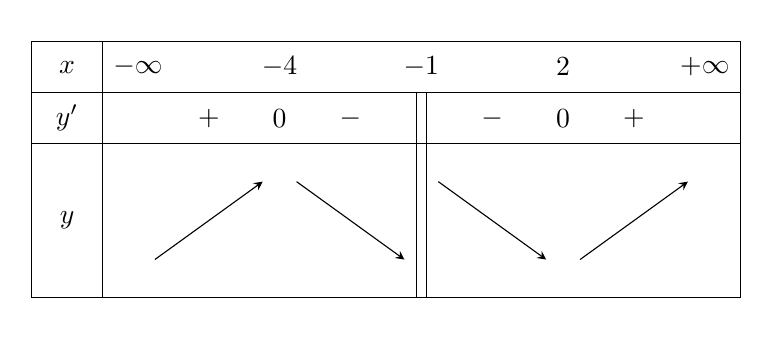
\begin{tikzpicture}[yscale=0.65,xscale=0.9]
 \def\c{9}%số cột
 \def\d{4}%số dòng
 \foreach \x in {0,...,\c}{
 \foreach \y in {0,...,\d}
 \path[yscale=-1] (\x,\y) node[gray!0,minimum size=1cm] (\x\y) {\x\y};
 }
 \draw[double,double distance=.12cm,shorten >=-0.83cm, shorten <=-0.18cm](50)--(54);
 \draw[shift={(-0.5,0.5)}]
 (0,0) rectangle (\c+1,-\d-1)
 (0,-1)--(\c+1,-1)
 (0,-2)--(\c+1,-2)
 (1,0)--(1,-\d-1);
 \path
 (00) node {$x$}(10) node {$-\infty$}(30) node {$-4$}(50) node {$-1$}(70) node {$2$}(90) node {$+\infty$}
 (01) node {$y'$}(21) node {$+$}(31) node {$0$}(41) node {$-$}(61) node {$-$}(71) node {$0$}(81) node {$+$}
 (03) node {$y$}
 ;
 \foreach \a/\b in {14/32,32/54,52/74,74/92}
 \draw[->,>=stealth,shorten >=-0.36cm, shorten <=-0.36cm] (\a)--(\b);
 \end{tikzpicture}
 \end{center}
 \item 	Dựa vào bảng biến thiên, hàm số nghịch biến trên $(-4 ;-1)$ và $ (-1 ; 2) $.
 \end{itemize}
 }
\end{ex}
%===27
\begin{ex}%[2D1B1-1]
 Hàm số $y=\sqrt{8+2x-x^2}$ đồng biến trên khoảng nào sau đây?
 \choice
 {$(1;+\infty)$}
 {$(1;4)$}
 {$(-\infty;1)$}
 {\True $(-2;1)$}
 \loigiai{
 \begin{itemize}
 \item $\mathscr{D}=[-2;4]$
 \item $y'=\dfrac{2-2x}{2\sqrt{8+2x-x^2}}=0\Leftrightarrow x=1$.
 \item Bảng biến thiên
 \begin{center}
 
\begin{tikzpicture}[>=stealth]
 \tkzTabInit[nocadre=false,lgt=1,espcl=3,deltacl=0.5]{$x$/.7 ,$y'$/.7,$y$/2}
 {$-2$ , $1$ , $4$}
 \tkzTabLine{ d, + , $0$ , - ,d }
 \tkzTabVar{-/ , +/ , -/}
 \end{tikzpicture}
 \end{center}
 \item Vậy hàm số nghịch biến trên khoảng $(-2;1)$.
 \end{itemize}
 }
\end{ex}
%Câu 57
\begin{ex}%[2D1Y1-2]
 \immini
 {
 Cho hàm số $ y=f(x) $ có đồ thị như hình vẽ bên. Hàm số đã cho đồng biến trên khoảng
 \choice
 {\True$(2;3)$}
 {$(0;2)$}
 {$(-2;1)$}
 {$(1;2)$}
 }
 {
 \begin{tikzpicture}[>=stealth,x=1cm,y=1cm,scale=0.5,font=\footnotesize]
 \path
 (0,0) coordinate (O)
 (-0.5,0) coordinate (A)
 %	Các điểm mút cho lệnh controls:
 (-1.5,3.3) coordinate (N)
 (1,1.6) coordinate (M1)
 (2.2,-0.8) coordinate (Q)
 (3.5,3.5) coordinate (M2)
 ;
 %Vẽ đường cong:
 %	\draw[red] (N)--(M1)--(Q)--(M2);
 \draw (N)..controls +(-80:0.5) and +(170:0.5)..(O)..controls +(10:0.5) and +(-170:0.25)..(M1)..controls +(-5:0.5) and +(175:0.5)..(Q)..controls +(5:0.5) and +(-100:0.25)..(M2);
 %Vẽ hệ trục tọa dộ:
 \draw[->] (-2,0)--(0,0) node[below left]{$O$}--(4.3,0) node[below]{$x$};
 \draw[->] (0,-1) --(0,4) node[left]{$y$};
 %	Vẽ nét đứt+node:
 \foreach \p/\n/\r in {N/-2/-90,M1/1/-90,Q/2/90,M2/3/-90}
 \draw[dashed](\p)--($(A)!(\p)!(O)$)node[shift={(\r:3mm)}]{$ \n $} ;
 \path ($(A)!(N)!(O)$)coordinate (A1) ($(A)!(M2)!(O)$)coordinate (B3)($(A)!(Q)!(O)$)coordinate (B2)($(A)!(M1)!(O)$)coordinate (B1);
 \foreach \p in {M1,M2,O,Q,N,A1,B3,B2,B1}
 \fill (\p) circle (1.7pt) ;
 \end{tikzpicture}
 }
 \loigiai{
 Dựa vào đồ thị, hàm số đồng biến trên các khoảng $ (0;1) $ và $ (2;3) $.
 }
\end{ex}
%Câu 59
\begin{ex}%[2D1Y1-2]
 \immini
 {
 Cho hàm số $ y=f(x) $ có đồ thị như hình vẽ bên. Hàm số đã cho đồng biến trên khoảng
 \choice
 {$(-2;4)$}
 {\True$(-2;1)$}
 {$(2;4)$}
 {$(-2;2)$}
 }
 {
 \begin{tikzpicture}[>=stealth,x=1cm,y=1cm,scale=0.4,font=\footnotesize]
 \path
 (0,0) coordinate (O)
 %	Các điểm mút cho lệnh controls:
 (-2,0) coordinate (A)node[below]{$ -2 $}
 (0,2) coordinate (D)node[left]{$ 2 $}
 (1,4.2) coordinate (M1)
 (2.5,3.5) coordinate (M2)
 (3.8,4.2) coordinate (M3)
 (5.3,2.5) coordinate (M4)
 ;
 %Vẽ đường cong:
 %	\draw[red] (A)--(D)--(M1)--(M2)--(M3)--(M4);
 \draw (A)..controls +(45:0.25) and +(-120:1)..(D)..controls +(60:0.5) and +(-170:0.25)..(M1)..controls +(10:0.35) and +(175:0.5)..(M2)..controls +(-5:0.25) and +(160:0.25)..(M3)..controls +(10:0.25) and +(120:0.25)..(M4);
 %Vẽ hệ trục tọa dộ:
 \draw[->] (-3,0)--(0,0) node[below left]{$O$}--(6,0) node[below]{$x$};
 \draw[->] (0,-1) --(0,5) node[left]{$y$};
 %	Vẽ nét đứt+node:
 \foreach \p/\n/\r in {M1/1/-90,M2/2/-90,M4/4/-90}
 \draw[dashed](\p)--($(A)!(\p)!(O)$)node[shift={(\r:3mm)}]{$ \n $} ;
 %	fill các điểm
 \path ($(A)!(M1)!(O)$)coordinate (B1)($(A)!(M2)!(O)$)coordinate (B2)($(A)!(M4)!(O)$)coordinate (B4);
 \foreach \p/\r in {M1,M2,M4,A,D,B1,B2,B4}
 \fill (\p) circle (1.7pt);
 \end{tikzpicture}
 }
 \loigiai{
 Dựa vào đồ thị, hàm số đồng biến trên khoảng $ (-2;1) $.
 }
\end{ex}
\begin{ex}%[2D1Y1-2]
 Cho hàm số $y=f(x)$ có bảng biến thiên như hình bên dưới. Hàm số đã cho đồng biến trên một đoạn có độ dài lớn nhất bằng
 \begin{center}
 \begin{tikzpicture}
 \tkzTabInit[lgt=1,espcl=2.5,deltacl=0.6]
 {$x$ /0.6,$y'$ /0.6,$y$ /1.8}
 {$-8$,$-1$,$2$,$4$,$8$}
 \tkzTabLine{,+,$0$,+,d,+,$0$,-,}
 \draw (N13)node[above](A){$-2$} ($(N13)!0.5!(N32) +(0,0.1)$) node(B){$1$} (N32)[below left]node(C){$+\infty$};
 \foreach \x/\y in {A/B,B/C}
 {\draw[-stealth] (\x)--(\y);}
 \draw[double] ([yshift=-0.5mm]N32)--(N33);
 \draw (N33)node[above right](D){$-\infty$} (N42)[below]node(E){$3$} (N53)[above]node(F){$-\infty$};
 \foreach \m/\n in {D/E,E/F}
 {\draw[-stealth] (\m)--(\n);}
 \end{tikzpicture}
 \end{center}
 \choice
 {$12$}
 {$7$}
 {$2$}
 {\True $10$}
 \loigiai{
 Từ bảng biến thiên ta có
 \begin{itemize}
 \item Hàm số đồng biến trên khoảng $(-8;2)$ và $(2;4)$.
 \item Hàm số nghịch biến trên khoảng $(4;8)$.
 \end{itemize}
 Khi đó hàm số đồng biến trên đoạn có độ dài lớn nhất sẽ bằng $10$.
 }
\end{ex}
\begin{ex}%[2D1Y1-2]
 Cho hàm số $y=f(x)$ có bảng biến thiên như hình bên dưới. Hàm số đã cho đồng biến trên khoảng nào?
 \begin{center}
 
\begin{tikzpicture}
 \tkzTabInit[lgt=1,espcl=2.5,deltacl=0.6]
 {$x$ /0.5,$y'$ /0.5,$y$ /1.5}
 {$-\infty$,$-1$,$0$,$1$,$+\infty$}
 \tkzTabLine{,-,$0$,+,$0$,-,$0$,+,}
 \tkzTabVar{+/$+\infty$, -/$-2$,+/$-1$,-/$-2$,+/$+\infty$}
 \end{tikzpicture}
 \end{center}
 \choice
 {$(-2;-1)$}
 {$(-1;1)$}
 {$(-\infty;-1)$}
 {\True $(-1;0)$}
 \loigiai{
 Từ bảng biến thiên ta có
 \begin{itemize}
 \item Hàm số đồng biến trên khoảng $(-1;0)$ và $(1;+\infty)$.
 \item Hàm số nghịch biến trên khoảng $(-\infty;-1)$ và $(0;1)$.
 \end{itemize}
 }
\end{ex}
\begin{ex}%[2D1B1-1]
 Hàm số $f(x$) có đạo hàm $f'(x)=x^2(x+1)^2(x+2),\forall x\in\mathbb{R}$. Khẳng định nào sau đây đúng?
 \choice
 {\True Hàm số đồng biến trên khoảng $(-2 ;+\infty)$}
 {Hàm số nghịch biến trên các khoảng$(-2 ;-1),(0 ;+\infty)$ }
 {Hàm số đồng biến trên khoảng $(-\infty,-2)$}
 {Hàm số đồng biến trên các khoảng $(-\infty ;-2),(0 ;+\infty)$}
 \loigiai
 {
 \begin{itemize}
 \item 	$f'(x)= x^2(x+1)^2(x+2)=0 \Leftrightarrow \hoac{&x=0 \text{ (loại)}\\ &x=-1 \text{ (loại)} \\ &x=-2.} $
 \item Bảng xét dấu $f'(x)$
 \begin{center}
 
\begin{tikzpicture}
 \tkzTabInit[nocadre=false,lgt=2,espcl=2,deltacl=0.5]{$x$/.7 ,$f'(x)$/.7}
 {$-\infty$ , $-2$ , $+\infty$}
 \tkzTabLine{ , - , 0 , + }
 \end{tikzpicture}
 \end{center}
 \item Vậy hàm số đồng biến trên khoảng $(-2 ;+\infty)$.
 \end{itemize}
 }
\end{ex}
\begin{ex}%[2D1B1-1]
 Cho hàm số $ y = f(x)$ có $f'(x)=\left(x^2-1\right)(x+1)(5-x), \forall x\in\mathbb{R}$. Mệnh đề nào sau đây đúng ?
 \choice
 {$f(1)<f(4)<f(2)$}
 {\True $f(1)<f(2)<f(4)$}
 {$f(2)<f(1)<f(4)$}
 {$f(4)<f(2)<f(1)$}
 \loigiai
 {
 \begin{itemize}
 \item $f'(x)=\left(x^2-1\right)(x+1)(5-x)=0 \Leftrightarrow \hoac{&x=-1\\ &x=1\\ &x=5.} $
 \item Bảng xét dấu $f'(x)$
 \begin{center}
 
\begin{tikzpicture}
 \tkzTabInit[nocadre=false,lgt=2,espcl=2,deltacl=0.5]{$x$/1 ,$f'(x)$/1 }
 {$-\infty$ , $-1$ , $1$ , $5$ , $+\infty$}
 \tkzTabLine{ , - , 0 , - , 0 , + , 0 , - }
 \end{tikzpicture}
 \end{center}
 \item 	Hàm số đồng biến trên khoảng $(1 ; 5)$. Vì vậy $f(1)<f(2)<f(4)$.
 \end{itemize}
 }
\end{ex}
\begin{ex}%[2D1Y1-2]
 Cho hàm số $y=f(x)$ xác định trên $\mathbb{R}$ và có bảng xét dấu đạo hàm như hình bên dưới. Mệnh đề nào dưới đây \textbf{đúng}?
 \begin{center}
 
\begin{tikzpicture}
 \tkzTabInit
 [nocadre=false,lgt=1.5,espcl=1.7,deltacl=0.6]
 {$x$/0.5, $y'$/0.5}
 {$-\infty$,$-2 $,$0 $,$2$,$+\infty$}
 \tkzTabLine{, + , 0 , - , d , - , 0 , + , }
 \end{tikzpicture}
 \end{center}
 \choice
 {Hàm số đồng biến trên khoảng $(-2;0 )$}
 {Hàm số đồng biến trên khoảng $(-\infty;0 )$}
 {\True Hàm số nghịch biến trên khoảng $(-2;2 )$}
 {Hàm số nghịch biến trên khoảng $(-\infty;-2)$}
 \loigiai
 {Dựa vào bảng xét dấu của đạo hàm, hàm số nghịch biến trên khoảng $(0;2 )$. }
\end{ex}
\begin{ex}%[2D1Y1-2]
 Cho hàm số $y=f(x)$ xác định trên $\mathbb{R}\setminus\{0 \}$ và có bảng xét dấu đạo hàm như hình bên dưới. Mệnh đề nào dưới đây \textbf{sai}?
 \begin{center}
 
\begin{tikzpicture}
 \tkzTabInit
 [nocadre=false,lgt=1.5,espcl=1.7,deltacl=0.6]
 {$x$/0.5, $y'$/0.5}
 {$-\infty$,$-1 $,$0 $,$3$,$+\infty$}
 \tkzTabLine{, + , $0$ , - , d , - , $0$ , + , }
 \end{tikzpicture}
 \end{center}
 \choice
 {Hàm số đồng biến trên khoảng $(-\infty;-1 )$}
 {Hàm số đồng biến trên khoảng $(3;+\infty )$}
 {Hàm số nghịch biến trên khoảng $(0;3)$}{\True Hàm số nghịch biến trên khoảng $(-1;3)$}
 \loigiai{Dựa vào bảng xét dấu đạo hàm và hàm số không xác định tại $x=0$ nên ta có hàm số không nghịch biến trên khoảng $(-1;3)$. }
\end{ex}
\begin{ex}%[2D1B1-2]
 \immini
 {
 Cho hàm số $f(x)$ xác định trên $\mathbb{R}$ và có đồ thị hàm số $y=f'(x)$ là đường cong trong hình vẽ bên dưới. Mệnh đề nào dưới đây đúng ?
 \choice
 {Hàm số $f(x)$ đồng biến trên khoảng $(1;2)$ }
 {Hàm số $f(x)$ đồng biến trên khoảng $(-2;1)$}
 {Hàm số $f(x)$ nghịch biến trên khoảng $(-1;1)$ }
 {\True Hàm số $f(x)$ nghịch biến trên khoảng $(0;2)$}
 }
 {
 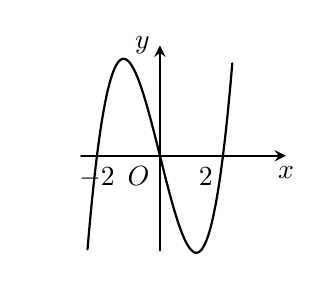
\begin{tikzpicture}[line join=round, line cap=round,>=stealth,thick,scale=0.4]
 \def \hamso{1*((\x)^3)-4*(\x)}
 \def \a{0} \def \b{1} \def \r{4}
 \tikzset{label style/.style={font=\footnotesize}}
 \draw[->] (-2.5,0)--(4,0) node[below] {$x$};
 \draw[->] (0,-3)--(0,3.5) node[left] {$y$};
 \draw (0,0) node [below left] {$O$};
 \draw (-2,1pt)--(-2,-1pt) node [below] {$-2$} (2,1pt)--(2,-1pt) node [below left] {$2$} ;
 \clip (\a-4.2,\b-4.2) rectangle (\a+\r,\b+\r-1);
 \draw[samples=200,domain=-2.3:2.3,smooth,variable=\x] plot (\x,{\hamso});
 \end{tikzpicture}
 }
 \loigiai
 {
 Dựa vào đồ thị ta thấy $f'(x)> 0 $ trên các khoảng $(-2;0), (2,+\infty)$ nên đồng biến trên các khoảng đó, $f'(x)<0$ trên các khoảng $(-\infty;-2), (0,2)$ nên nghịch biến trên các khoảng đó.
 }
\end{ex}
\begin{ex}%[2D1B1-2]
 \immini{Cho hàm số $y=f(x)$ có đồ thị $y=f'(x)$ là một parabol được cho như hình vẽ . Hàm số $y=f(x)$ nghịch biến trên khoảng nào dưới đây?
 \choicew{0.4\textwidth}
 \choice
 {$(1;3)$}
 {$(4;3)$}
 {\True $(3;+\infty)$}
 {$(1;+\infty)$}
 }
 {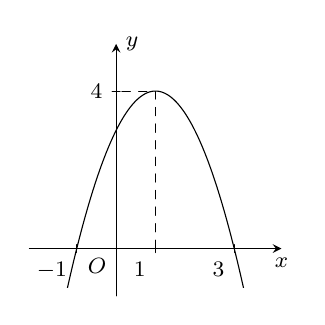
\begin{tikzpicture}[scale=0.5, font=\footnotesize, line join=round, line cap=round, >=stealth]
 \def\xmin{-2}\def\xmax{4}\def\ymin{-1}\def\ymax{5}
 \draw[->] (\xmin-0.2,0)--(\xmax+0.2,0) node[below] {\footnotesize $x$};
 \draw[->] (0,\ymin-0.2)--(0,\ymax+0.2) node[right] {\footnotesize $y$};
 \draw (0,0) node [below left] {\footnotesize $O$};
 \foreach \x in {-1,1,3}\draw (\x,0.1)--(\x,-0.1) node [below left] {\footnotesize $\x$};
 \foreach \y in {4}\draw (0.1,\y)--(-0.1,\y) node [left] {\footnotesize $\y$};
 \clip (\xmin,\ymin) rectangle (\xmax,\ymax);
 \draw[dashed] (1,0)--(1,4)--(0,4);
 \draw[smooth,samples=200,domain=\xmin:\xmax] plot (\x,{-1*((\x)^2)+2*\x+3});
 \end{tikzpicture} }
\end{ex}
\begin{ex}%[2D1B1-2]
 \immini
 {
 Cho hàm số $ y=f(x) $ xác định và liên tục trên $ [-2;3] $ đồng thời hàm số $ y=f'(x) $ có đồ thị như hình vẽ bên. Hàm số đã cho đồng biến trên khoảng nào sau đây?
 \choice
 {\True $(1;2)$}
 {$(0;1)$}
 {$(2;3)$}
 {$(-2;2)$}
 }
 {
 \begin{tikzpicture}[>=stealth,scale=0.7,font=\footnotesize]
 \path
 (0,0) coordinate (O)
 (-2.5,0) coordinate (A1)
 (-1.75,1) coordinate (N)
 (0.2,-2) coordinate (Q1)
 (1.75,1) coordinate (M)
 (3.5,-3) coordinate (Q2)
 ;
 \draw[name path=fx] (A1)..controls +(70:0.25) and +(-180:0.25)..(N)..controls +(0:0.5) and +(180:0.65)..(Q1)..controls +(5:0.5) and +(-180:0.65)..(M)..controls +(-0:0.65) and +(120:0.25)..(Q2)node[black,shift={(-0.7,0.2)}]{$ y=f'(x) $};
 \draw [domain=-3:3, samples=0.1,name path=gx] plot (\x, 0);
 \path[name intersections={of=fx and gx, by={-2,-1,1,2}}] ;
 \draw[->] (-3,0)--(0,0) node[below left]{$O$}--(4,0) node[below]{$x$};
 \draw[->] (0,-3.2) --(0,1.5) node[left]{$y$};
 \foreach \p/\r in {-2/-120,-1/-120,1/120,2/60}
 \draw[fill=black] (\p) circle (1.2pt) node[shift={(\r:2.5mm)}]{$\p$};
 \draw[dashed](Q2)--($(A1)!(Q2)!(O)$)node[above]{$ 3 $};
 \end{tikzpicture}
 }
 \loigiai{
 Dựa vào đồ thị $ y=f'(x) $, hàm số đồng biến trên các khoảng $ (-2;-1) $ và $ (1;2) $, nghịch biến trên các khoảng $ (-1;1) $ và $ (2;3) $.
 }
\end{ex}
\begin{ex}%[2D1K1-1]
 Cho hàm số $y=\sqrt{2x-x^2}-x$. Hỏi hàm số nghịch biến trên khoảng nào sau đây?
 \choice
 {$(0 ; 1)$}
 {$(-\infty, 1)$}
 {$(1 ;+\infty)$}
 {\True $(1 ; 2)$}
 \loigiai
 {
 \begin{itemize}
 \item $\mathscr{D}=[0;2]$.
 \item $y'=\dfrac{-x+1}{\sqrt{2x-x^2}}-1=0\Leftrightarrow x=\dfrac{2-\sqrt{2}}{2}$.
 \item Bảng biến thiên
 \begin{center}
 
\begin{tikzpicture}[>=stealth]
 \tkzTabInit[nocadre=false,lgt=1,espcl=3,deltacl=0.5]{$x$/1.2,$y'$/.7,$y$/2}
 {$0$ , $\dfrac{2-\sqrt{2}}{2}$ , $2$}
 \tkzTabLine{ d, + , $0$ , - ,d }
 \tkzTabVar{-/, +/, -/}
 \end{tikzpicture}
 \end{center}
 \item 	Vậy hàm số đã cho đồng biến trên khoảng $\left(0;\dfrac{2-\sqrt{2}}{2}\right)$, nghịch biến trên $\left(\dfrac{2-\sqrt{2}}{2};2\right)$.
 \end{itemize}
 }
\end{ex}
\begin{ex}%[2D1K1-1]
 Cho hàm số $f(x)=x^3+8x+\cos5x$. Với hai số thực $a<b$, khẳng định nào sau đây đúng?
 \choice
 {$f(a)=f(b)$}
 {$f(a)>f(b)$}
 {\True $f(a)<f(b)$}
 {$f(a)\ge f(b)$}
 \loigiai{
 \begin{itemize}
 \item $\mathscr{D} = \mathbb{R}$
 \item $f'(x)=3x^2+8-5\sin5x \Rightarrow f'(x)>0, \forall x \in \mathscr{D}$.
 \item Hàm số luôn đồng biến trên $\mathbb{D}=\mathbb{R}$. Vì vậy $a<b \Rightarrow f(a)<f(b)$
 \end{itemize}
 }
\end{ex}
\BTTF
\begin{ex}%[EX-TF-2024, Lê Quốc Hiệp]%[2D1N1-2]
    Cho hàm số $y = f(x)$ có đạo hàm liên tục trên $\mathbb{R}$ và có bảng biến thiên như hình bên dưới. Xét tính đúng, sai của các mệnh đề sau
    \begin{center}
        
\begin{tikzpicture}
            \tkzTabInit[nocadre=false,lgt=1.2,espcl=2.5,deltacl=0.6]
            {$x$ /0.6,$y’$ /0.6,$y$ /2}
            {$-\infty$,$-1$,$0$,$1$,$+\infty$}
            \tkzTabLine{ ,-,$0$,+,$0$,-,$0$,+, }
            \tkzTabVar{+/$+\infty$,-/$-4$,+/$-3$,-/$-4$,+/$+\infty$}
        \end{tikzpicture}
    \end{center}
    \choiceTF
    {\True Hàm số đã cho đồng biến trên $ (-1; 0) $}
    {Hàm số đã cho đồng biến trên $ (-4; -3) $}
    {\True Hàm số đã cho đồng biến trên $ (1;+\infty) $}
    {Hàm số đã cho đồng biến trên $ (0; 1) $}
    \loigiai{
        Dựa vào bảng biến thiên suy ra hàm số $y=f(x)$ đồng biến trên các khoảng $(-1;0)$ và $(1;+\infty)$.
    }
\end{ex}
\begin{ex}%[EX-TF-2024, Lê Quốc Hiệp]%[2D1N1-2]
    \immini{Cho hàm số $y=f(x)$ có đồ thị như hình vẽ bên. Xét tính đúng, sai của mỗi mệnh đề sau
        \choiceTF
        {\True Hàm số nghịch biến trên $(0;2)$}
        {Hàm số nghịch biến trên $(-2;2)$}
        {Hàm số nghịch biến trên $(-\infty;0)$ và $(2;+\infty)$
        }
        {Với mọi $x\in (0;2)$ thì hàm số luôn nhận giá trị dương}
    }{
        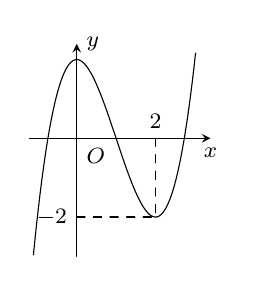
\begin{tikzpicture}[scale=1, font=\footnotesize, line join=round, line cap=round, >=stealth]
            \draw[->] (-0.6,0)--(1.7,0) node[below]{$x$};
            \draw[->] (0,-1.5)--(0,1.2) node[right]{$y$};
            \node at (0,0) [below right]{$O$};
            \node at (0,-1) [left]{\footnotesize $-2$};	\node at (1,0) [above]{\footnotesize $2$};
            \draw[domain=-0.55:1.51, samples=100] plot(\x,{4*(\x)^3-6*(\x)^2+1});
            \draw[dashed] (0,-1)--(1,-1)--(1,0);
        \end{tikzpicture}
    }
    \loigiai{
        Dựa vào đồ thị suy ra hàm số $y=f(x)$ đồng biến trên các khoảng $(-1;0)$ và $(2;+\infty)$.
    }
\end{ex}
\begin{ex}
 Cho hàm số $y=x^4-2x^2+2$. Xét tính đúng, sai của các mệnh đề sau
 \choiceTF
 {Tập xác định của hàm số là $D=\left[ 0;+\infty \right)$}
 {Hàm số đồng biến trên khoảng $(-2;0)$}
 {Hàm số đồng biến trên $\left( -\dfrac{1}{2};+\infty\right)$}
 {Hàm số nghịch biến trên các khoảng $(-\infty;-1)$ và $(0;1)$}
\end{ex}
\begin{ex}
 Cho hàm số $y=\dfrac{x-1}{x+2}$. Xét tính đúng, sai của mỗi khẳng định sau
 \choiceTF
 {Tập xác định của hàm số là $D=\mathbb{R}$}
 {Hàm số nghịch biến trên $\mathbb{R}\setminus\{-2\}$}
 {Hàm số đồng biến trên $\mathbb{R}\setminus\{-2\}$}
 {\True Hàm số đồng biến trên $(-\infty;-2)$ và $(-2;+\infty)$}
\end{ex}
\begin{ex}
    Cho hàm số $y=\dfrac{-x^2+2x-1}{x+2}$. Xét tính đúng, sai của các mệnh đề sau
    \choiceTF
    {Tập xác định của hàm số là $\mathbb{D}=\mathbb{R}\setminus\{-2\}$}
    {Phương trình $y'=0$ có hai nghiệm nguyên dương}
    {Hàm số đồng biến trên $(-5;-2)$ và $(-2;+\infty)$}
    {Hàm số nghịch biến trên $(-\infty;-5)$ và $(1;+\infty)$}
\end{ex}
%===== DẠNG 2

\BTTL
\begin{ex}\immini{Cho hàm số $y=f\left(x\right)$ liên tục trên đoạn $\left[-3;3\right]$ và có đồ thị như hình bên. Tìm các khoảng đơn điệu của hàm số $f\left(x\right)$ trên khoảng $\left(-3;3\right)$.
     \shortans{}
 } {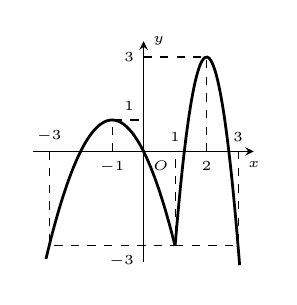
\begin{tikzpicture}[>=stealth,scale=0.4,font=\tiny]
 \draw[->] (-3.5,0) --(0,0) node[below
 right]{$O$} -- (3.5,0)
 node[below]{$x$};
 \draw[->](0,-3.5)--(0,3.5)
 node[right]{$y$};
 \draw[dashed] (-3,0)node[above]{$-3$}--(-1,0)node[below]{$-1$}--(1,0)node[above]{$1$}--(2,0)node[below]{$2$}--(3,0)node[above]{$3$};
 \draw (0,-3) node[below left]{$-3$} --(0,1)node[above left ]{$1$}--(0,3)node[left]{$3$};
 \draw[smooth,line width=1]
 plot[domain=-3.1:1]
 (\x,{-(\x)^2-2*(\x)});
 \draw[smooth,line width=1]
 plot[domain=1:3.05]
 (\x,{-6*(\x)^2+24*(\x)-21});
 \draw[dashed] (-3,0)--(-3,-3)--(0,-3)--(1,-3)--(1,0) ;
 \draw[dashed](1,-3)--(3,-3)--(3,0);
 \draw[dashed] (-1,0)--(-1,1)--(0,1);
 \draw[dashed] (2,0)--(2,3)--(0,3);
 \end{tikzpicture}}
 \loigiai{
 \begin{itemize}
 \item Với $x \in \left(-3;1\right)\subset \left(-3;3\right)$. Hàm số đạt cực đại tại $x=-1$ và giá trị cực đại $f_{\text{CĐ}}=1$.
 \item Với $x \in \left(1;3\right)\subset \left(-3;3\right)$. Hàm số đạt cực đại tại $x=2$ và giá trị cực đại $f_{\text{CĐ}}=3$.
 \end{itemize}
 }
\end{ex}
\begin{ex}
 Xác định các khoảng đơn điệu của hàm số $y=f(x)$ liên tục trên các khoảng $\left(-\infty;1\right)$, $\left(1;+\infty\right)$ các có bảng biến thiên như sau
 \begin{center}
 
\begin{tikzpicture}[>=stealth]
 \tkzTabInit[nocadre=false,lgt=1.5,espcl=2,deltacl=0.6]{$x$/.6 ,$f'(x)$/.6,$f(x)$/2}
 {$-\infty$ ,$1$ , $2$ , $3$, $4$, $5$ , $+\infty$}
 \tkzTabLine{ , + , d , - , $0$ , + ,$0$ , + ,d, - ,$0$ , + , }
 \tkzTabVar{-/$-\infty$, +D+/$\infty$/$+\infty$,-/$-2$,R,+/$1$,-/$-1$, +/$+\infty$}
 \end{tikzpicture}
 \end{center}
 \shortans{}
 \loigiai{
 Dựa vào bảng biến thiên, ta thấy
 \begin{itemize}
 \item Hàm số đồng biến trên các khoảng $(-\infty;1)$; $(2;4)$ và $(5;+\infty)$.
 \item Hàm số nghịch biến trên các khoảng $(1;2)$ và $(4;5)$.
 Hàm số đạt cực tiểu tại $x=2$ và $x=5$.
 \item Hàm số nghịch biến trên các khoảng $(1;2)$ và $(4;5)$.
 Hàm số đạt cực đại tại $x=4$.
 \end{itemize}
 }
\end{ex}
\begin{ex}%[Dự án Tex hóa SKG KNTT - Nguyễn Mạnh Trung Anh]%[2D1H2-2]
 \immini
 {
 Đồ thị của đạo hàm bậc nhất $y=f'(x)$ của hàm số $f(x)$ được cho trong hình vẽ bên dưới. Hãy tìm các khoảng đồng biến của hàm số $y=f(x)$
 }
 {
 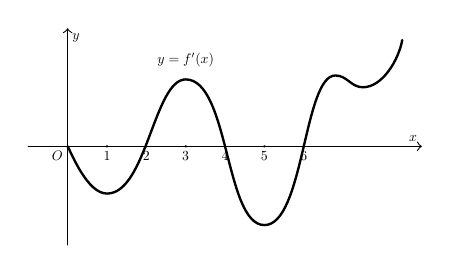
\begin{tikzpicture}[line join=round, line cap=round,transform shape,scale=0.5]
 \def\xmin{-1} \def\xmax{9}
 \def\ymin{-2.5} \def\ymax{3}
 \draw[->] (\xmin,0)--(\xmax,0) node [above left]{$x$};
 \draw[->] (0,\ymin)--(0,\ymax) node [below right]{$y$};
 \node at (0,0) [below left]{$O$};
 \node at (3,2.2) {$y=f'(x)$};
 \foreach \x in{1,2,3,4,5,6}\draw[fill=black] (\x,0) circle (.5pt) node[below]{$\x$};
 \clip (\xmin+0.1,\ymin+0.1) rectangle (\xmax-0.1,\ymax-0.1);
 \draw[line width=.3mm, black] (0,0)
 ..controls +(-60:.2) and +(180:.5) ..(1,-1.2)
 ..controls +(0:1) and +(180:.8) ..(3,1.7)
 ..controls +(0:1.1) and +(180:1) ..(5,-2)
 ..controls +(0:1) and +(180:.8) ..(6.8,1.8)
 ..controls +(0:.3) and +(180:.3) ..(7.5,1.5)
 ..controls +(0:.5) and +(-100:.5) ..(8.5,2.7)
 ;
 \end{tikzpicture}
 }
 \shortans{}
 \loigiai{
 \begin{enumerate}
 \item Từ đồ thị hàm số, ta có $f'(x)>0\Leftrightarrow\heva{&x\in(2;4)\\&x\in(6;+\infty).}$ và liên tục trên hai khoảng đó.\\
 Do đó hàm số $f(x)$ đồng biến trên $(2;4)$ và $(6;+\infty)$.
 \item Từ đồ thị hàm số, ta có $f'(x)=0\Leftrightarrow\heva{&x=2\\&x=4\\&x=6}$ và qua các điểm đó thì $f'(x)$ đổi dấu.\\
 Vậy tại các điểm $x=2$, $x=4$, $x=6$ thì hàm số $f(x)$ có cực đại hoặc cực tiểu.
 \end{enumerate}
 }
\end{ex}
\begin{ex}
    \immini{Cho hàm số $y=f(x)$ liên tục trên đoạn $[0 ; 3]$ thoả mãn $f^{\prime}\left(\dfrac{1}{3}\right)=f^{\prime}(1)=f^{\prime}\left(\dfrac{5}{2}\right)=0$ và có đồ thị là đường cong như hình bên. Xác định các khoảng đơn điệu và tìm cực trị của hàm số đã cho trên khoảng $(0;3)$.}{\begin{tikzpicture}[line cap=butt,line join=miter,>=stealth,font=\footnotesize,scale=.7]
            \tikzset{declare function={xmin=-2;xmax=4;ymin=-3;ymax=2;
                    f(\x)=32/45*(\x)^4-32/9*(\x)^3+224/45*(\x)^2-32/15*(\x);
                },
                smooth,samples=450
            }
            \draw[->] (xmin,0)--(xmax,0) node[shift={(-100:7pt)}]{$ x $};
            \draw[->] (0,ymin)--(0,ymax) node[shift={(190:7pt)}]{$ y $};
            \fill (0,0) node[shift={(135:10pt)}]{$ O $};
            \draw[dashed](1/3,0)node[shift={(90:8pt)}]{$\tfrac{1}{3}$}|-(0,-1/3)node[shift={(-150:9pt)}]{$-\tfrac{1}{3}$}
            (2.5,0)node[shift={(90:7pt)}]{$\tfrac{5}{2}$}|-(0,-2)node[shift={(180:9pt)}]{$-2$}	(1,0)node[shift={(90:7pt)}]{$1$};
            \clip (xmin,ymin) rectangle (xmax,ymax);
            \draw plot[domain=xmin:xmax] (\x, {f(\x)});
    \end{tikzpicture}}
    \shortans{}
    \loigiai{Bảng biến thiên
        \begin{center}
            
\begin{tikzpicture}
                \tkzTabInit
                {$x$/.7,$f'(x) $/.7,$f(x)$/2}
                {$-\infty$,$\tfrac{1}{3}$,$1$,$\tfrac{5}{2}$,$+\infty$}
                \tkzTabLine{,-,0,+,0,-,0,+,}
                \tkzTabVar{+/$+\infty$,-/, +/,-/, +/$+\infty$}
            \end{tikzpicture}
        \end{center}
        Từ bảng biến thiên, suy ra
        \begin{itemize}
            \item $x=1$ là điểm cực đại của hàm số.
            \item $x=\dfrac{1}{3}$, $x=\dfrac{5}{2}$ là điểm cực tiểu của hàm số.
            \item Hàm số đã cho đồng biến trên $\left(\dfrac{1}{3};1\right)$, $\left(\dfrac{5}{2};+\infty\right)$, nghịch biến trên $\left(-\infty;\dfrac{1}{3}\right)$, $\left(1;\dfrac{5}{2}\right)$.
    \end{itemize}}
\end{ex}
\begin{ex}%[2D1N1-2]
 Tìm các khoảng đồng biến, khoảng nghịch biến của các hàm số có đồ thị như sau:
\begin{listEX}[2]
    \item  \begin{tikzpicture}[scale=1,xscale=1.3, font=\footnotesize, line join=round, line cap=round, >=stealth]
           \draw[gray!50,thin,opacity=.5] (-2,-2) grid (3,3);
           \draw[->] (-1.6,0)--(2.6,0) node[below] {$x$};
           \draw[->] (0,-1.5)--(0,2.6) node[left] {$y$};
           \draw (0,0) node [above left] {$O$};
           \foreach \x/\nx in {-1/-1,1/1,2/2}
           \draw[thin] (\x,1pt)--(\x,-1pt) node [above] {$\nx$};
           \foreach \y/\ny in {1/1,2/2}
           \draw[thin] (1pt,\y)--(-1pt,\y) node [left] {$\ny$};
           \begin{scope}
               \clip (-2.8,-2) rectangle (4,4);
               \draw[samples=200,domain=-0.8:2,smooth] plot (\x,{(\x)^3-1.5*(\x)^2});
           \end{scope}
           \draw[dashed,thin] (0,-0.5)node[left]{$-\tfrac{1}{2}$}--(1,-0.5)--(1,0);
           \draw (1.2,0) node[below right]{$1,5$};
   \end{tikzpicture}
\item  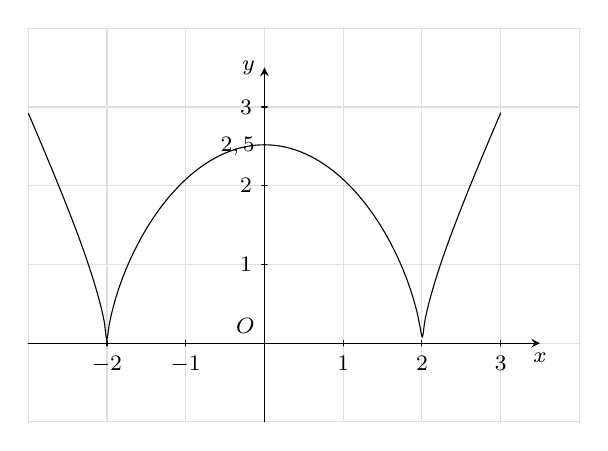
\begin{tikzpicture}[scale=1, font=\footnotesize, line join=round, line cap=round, >=stealth]
    \draw[gray!50,thin,opacity=.5] (-3,-1) grid (4,4);
    \draw[->] (-3,0)--(3.5,0) node[below] {$x$};
    \draw[->] (0,-1)--(0,3.5) node[left] {$y$};
    \draw (0,0) node [above left] {$O$};
    \foreach \x/\nx in {-2/-2,-1/-1,1/1,2/2,3/3}
    \draw[thin] (\x,1pt)--(\x,-1pt) node [below] {$\nx$};
    \foreach \y/\ny in {1/1,2/2,3/3}
    \draw[thin] (1pt,\y)--(-1pt,\y) node [left] {$\ny$};
    \begin{scope}
        %\clip (-3,-1) rectangle (2.9,1.2);
        \draw[samples=200,domain=3:-3,smooth] plot (\x,{(((\x)^2-4)^2)^(1/3)});
    \end{scope}
    \draw[dashed,thin] (0,2.5)node[left]{$2,5$};
\end{tikzpicture}
\end{listEX}
 \shortans{}
 \loigiai{
 \begin{enumerate}[a)]
 \item Quan sát đồ thị \textit{Hình} $H.1.11$, ta thấy hàm số $y=x^3-\dfrac{3}{2}x^2$ đồng biến trên các khoảng $(-\infty;0)$, $(1;+\infty)$; nghịch biến trên khoảng $(0;1)$.
 \item Quan sát đồ thị \textit{Hình} $H.1.12$, ta thấy hàm số $y=\sqrt[3]{\left(x^2-4\right)^2}$ đồng biến trên các khoảng $(-2;0)$, $(2;+\infty)$; nghịch biến trên các khoảng $(-\infty;-2)$, $(0;2)$.
 \end{enumerate}
 }
\end{ex}
\begin{ex} Cho hàm số $y=f\left(x\right)$ có đạo hàm là $y'=f'\left(x\right)=x\left(x-1\right)^2\left(x+3\right),\forall x \in \mathbb{R}$. Xác định các khoảng đồng biến, nghịch biến của hàm số $f\left(x\right)$ đã cho.
 \shortans{}
 \loigiai{Ta có $y'=f'\left(x\right)=0\Leftrightarrow \hoac{&x=0\\&x=1\\&x=-3.}$\\
 Bảng biến thiên \begin{center}
 
\begin{tikzpicture}
 \tkzTabInit[lgt=1.2,espcl=3]
 {$x$ /.7, $f’(x)$ /.7}
 {$-\infty$,$-3$,$0$,$1$,$+\infty$}
 \tkzTabLine{ ,+,z,-,z,+,z,+}
 %	\tkzTabVar{-/$-\infty$,+/$f(x_1)$,-/$f(x_2)$,+/$+\infty$}
 \end{tikzpicture}
 \end{center}
 Vậy hàm số đồng biến trên khoảng $\left(-\infty,-3\right)$ và $\left(0,+\infty\right)$, hàm số nghịch biến trên khoảng $\left(-3,0\right)$.
 }
\end{ex}
\begin{ex}%[2D1V1-5]
 Thể tích $V$ (đơn vị: centimét khối) của $1$ kg nước tại nhiệt độ $T\left(0^{\circ}\mathrm{C}\leq T \leq 30^{\circ}\mathrm{C}\right)$ được tính bởi công thức sau:
 $$V(T)=999{,}87-0{,}06426T+0{,}0085043T^2-0{,}0000679T^3.$$
 Hỏi thể tích $V(T), 0^{\circ}\mathrm{C}\leq T \leq 30^{\circ}\mathrm{C}$, giảm trong khoảng nhiệt độ nào?
 \shortans{$0^\circ$C đến $3{,}966514624^\circ$C}
 \loigiai{
 Xét hàm số $V(T)=999{,}87-0{,}06426T+0{,}0085043T^2-0{,}0000679T^3$, với $T\in [0;30]$.\\
 Ta có $V'(T)=-0{,}0002037T^2+0{,}0170086T-0{,}06426$.\\
 $V'(T)=0\Leftrightarrow T=3{,}966514624=T_1$ hoặc $T=79{,}53176716\not\in [0;30]$.\\
 Bảng biến thiên của hàm số $V(T)$ như sau
 \begin{center}
 
\begin{tikzpicture}[font=\footnotesize,thick,>=stealth]
 \tikzset{double style/.append style={double distance=1.5pt}}
 \tkzTabInit[nocadre=false,lgt=1.2,espcl=2.5,deltacl=0.6,lw=.75pt,color,colorL=green!50,colorV=green!50]
 {$T$ /0.7, $V'(T)$ /0.8, $V(T)$ /2}
 {$0$,$T_1$,$30$}
 \tkzTabLine{ ,-,$0$,+, }
 \tkzTabVar{+/$V(0)$,-/$V(T_1)$,+/$V(30)$}
 \end{tikzpicture}
 \end{center}
 Từ bảng biến thiên suy ra, thể tích $V(T), 0^{\circ}\mathrm{C}\leq T \leq 30^{\circ}\mathrm{C}$, giảm trong khoảng nhiệt độ từ $0^\circ$C đến $3{,}966514624^\circ$C.
 }
\end{ex}
\begin{ex}%[2D1V1-5]
 Kính viễn vọng không gian Hubble được đưa vào vũ trụ ngày 24/4/1990 bằng tàu con thoi Discovery. Vận tốc của tàu con thoi trong sứ mệnh này, từ lúc cất cánh tại thời điểm $t=0$ (s) cho đến khi tên lửa đẩy được phóng đi tại thời điểm $t=126$ (s), cho bởi công thức sau:
 $$
 v(t)=0{,}001302t^3-0{,}09029t^2+23,
 $$
 \centerline{
 ($v$ được tính bằng ft/s, 1 feet $=0{,}3048 \mathrm{~m}$)}\\
 Hỏi gia tốc của tàu con thoi sẽ tăng trong khoảng thời gian nào tính từ thời điểm cất cánh cho đến khi tên lửa đẩy được phóng đi?
 \shortans{$23{,}11571941$ s đến $126$ s}
 \loigiai{
 Gia tốc của tàu con thoi là $a(t)=v'(t)=0{,}003906t^2-0{,}18058t$.\\
 Xét hàm số $a(t)=0{,}003906t^2-0{,}18058t$ với $t\in [0;126]$.\\
 Ta có $a'(t)=0{,}007812t-0{,}18058$;\\
 $a'(t)=0\Leftrightarrow t=23{,}11571941=t_0$.\\
 Bảng biến thiên của hàm số $a(t)$ như sau
 \begin{center}
 
\begin{tikzpicture}[font=\footnotesize,thick,>=stealth]
 \tikzset{double style/.append style={double distance=1.5pt}}
 \tkzTabInit[nocadre=false,lgt=1.2,espcl=2.5,deltacl=0.6,lw=.75pt,color,colorL=green!50,colorV=green!50]
 {$t$ /0.7, $a'(t)$ /0.8, $a(t)$ /2}
 {$0$,$t_0$,$126$}
 \tkzTabLine{ ,-,$0$,+, }
 \tkzTabVar{+/$a(0)$,-/$a(t_0)$,+/$a(126)$}
 \end{tikzpicture}
 \end{center}
 Từ bảng biến thiên suy ra, gia tốc của tàu con thoi sẽ tăng trong khoảng thời gian từ $23{,}11571941$ s đến $126$ s.
 }
\end{ex}
\begin{ex}%[TeX hóa SGK CTST 12]%[Nguyễn Tiến]%[2D1H1-5]
 Kim ngạch xuất khẩu rau quả của Việt Nam trong các năm từ $2010$ đến $2017$ có thể được tính xấp xỉ bằng công thức $f(x)=0{,}01x^3-0{,}04x^2+0{,}25x+0{,}44$ (tỉ USD) với $x$ là số năm tính từ $2010$ đến $2017$ $(0\leq x\leq 7)$. Tìm khoảng thời gian mà kim ngạch xuất khẩu rau quả của Việt Nam liên tục tăng.
% \begin{flushright}
% (\textit{Theo:} https://infographics.vn/interactive-xuat-khau-rau-qua-\\
% du-bao-bung-no-dat-4-ty-usd-trong-nam-2023/116220.vna)
% \end{flushright}
% \begin{enumerate}
% \item Tính đạo hàm của hàm số $y=f(x)$.
% \item Chứng minh rằng kim ngạch xuất khẩu rau quả của Việt Nam tăng liên tục trong các năm từ $2010$ đến $2017$.
% \end{enumerate}
\shortans{$2010$ đến $2017$.}
 \loigiai{
 \begin{enumerate}
 \item Ta có $f'(x)=0{,}03x^2-0{,}08x+0{,}25$.
 \item Xét $f'(x)=0 \Leftrightarrow 0{,}03x^2-0{,}08x+0{,}25=0$ (vô nghiệm).\\
 Bảng biến thiên
 \begin{center}
 
\begin{tikzpicture}
 \tkzTabInit[nocadre=true,lgt=1.2,espcl=5,deltacl=0.6]
 {$x$ /0.6,$f'(x)$ /0.6,$f(x)$ /2}
 {$0$,$7$}
 \tkzTabLine{,+,}
 \tkzTabVar{-/$0{,}44$,+/$3{,}66$}
 \end{tikzpicture}
 \end{center}
 Từ bảng biến thiên trên, ta thấy $f(x)>0$, $\forall x\in [0;7]$.\\
 Vậy kim ngạch xuất khẩu rau quả của Việt Nam tăng liên tục trong các năm từ $2010$ đến $2017$.
 \end{enumerate}
 }
\end{ex}
%==================bài 6==================
\begin{ex}%[TeX hóa SGK CTST 12]%[Nguyễn Tiến]%[2D1V1-5]
 Xét một chất điểm chuyển động dọc theo trục $Ox$. Toạ độ của chất điểm tại thời điểm $t$ được xác định bởi hàm số $x(t)=t^3-6t^2+9t$ với $t\geq 0$. Khi đó $x'(t)$ là vận tốc của chất điểm tại thời điểm $t$, kí hiệu $v(t)$; $v'(t)$ là gia tốc chuyển động của chất điểm tại thời điểm $t$, kí hiệu $a(t)$. Trong khoảng thời gian nào vận tốc của chất điểm tăng, trong khoảng thời gian nào vận tốc của chất điểm giảm?
% \begin{enumerate}
% \item Tìm các hàm $v(t)$ và $a(t)$.
% \item Trong khoảng thời gian nào vận tốc của chất điểm tăng, trong khoảng thời gian nào vận tốc của chất điểm giảm?
% \end{enumerate}
\shortans{vận tốc của chất điểm tăng khi $t\in (0;1) \cup (3;+\infty)$, và giảm khi $t\in (1;3)$.}
 \loigiai{
 \begin{enumerate}
 \item Ta có $v(t)=x'(t)=3t^2-12t+9$ và $a(t)=v'(t)=6t-12$.
 \item Xét $v(t)=0 \Leftrightarrow \hoac{& t=1\\& t=3.}$\\
 Bảng xét dấu
 \begin{center}
 
\begin{tikzpicture}
 \tkzTabInit[nocadre=false,lgt=2,espcl=2.1]
 {$t$ /0.6,$v(t)$ /0.6}
 {$0$,$1$,$3$,$+\infty$}
 \tkzTabLine{,+,$0$,-,$0$,+,}
 \end{tikzpicture}
 \end{center}
 Suy ra vận tốc của chất điểm tăng khi $t\in (0;1) \cup (3;+\infty)$, và giảm khi $t\in (1;3)$.
 \end{enumerate}
 }
\end{ex}

%%%=============BT_6=============%%%
%%%=============BT_7=============%%%
\begin{ex} Thể tích $V$ của $1$ kg nước (tính bằng $\text{cm}^3$) ở nhiệt độ $T$ (đơn vị: $\circ C$) khi $T$ thay đổi từ $^\circ C$ đến $30^\circ C$ được cho xấp xỉ bởi công thức:
 $$V=999{,}87-0{,}06426T+0,0085043T^2-0{,}0000769T^3.$$
 Tìm nhiệt độ $T_0 \in \left(0;30\right)$ để kể từ nhiệt độ $T_0$ trở lên thì thể tích $V$ tăng (làm tròn kết quả đến hàng đơn vị).
 \shortans{}
 \loigiai{Xét hàm số $f\left(T\right)=V=999{,}87-0{,}06426T+0,0085043T^2-0{,}0000769T^3$.\\ Hàm số xác định trên khoảng $\left(0;30\right)$\\
 Ta có $f'\left(T\right)=2{,}307 \cdot 10^{-4}T^2+0{,}0170086T-0{,}06426$.\\
 $f'\left(T\right)=0\Leftrightarrow \hoac{&x=3{,}6\\&x=-77{,}33}\Leftrightarrow x=3{,}6$.
 \begin{center}
 
\begin{tikzpicture}
 \tkzTabInit[lgt=1.2,espcl=3]
 {$T$ /.7, $f’(T)$ /.7, $f(T)$ /2.5}
 {$0$,$3{,}6$,$30$}
 \tkzTabLine{ ,-,z,+,}
 \tkzTabVar{+/$f\left(0\right)$,-/$f\left(3{,}6\right)$,+/$f\left(30\right)$}
 \end{tikzpicture}
 \end{center}
 Vậy $T_0=4^\circ C$ trở lên thì nhiệt độ tăng.
 }
\end{ex}
\begin{ex} Xét tính đơn điệu của hàm số $y=f\left(x\right)=\sin x-x$ trên khoảng $\left(-\pi,\pi\right)$.
 \shortans{Nghịch biến trên $\left(-\pi,\pi\right)$}
 \loigiai{
 Hàm số đã cho xác định trên $\left(-\pi,\pi\right)$.\\
 Ta có $y'=f'\left(x\right)=\cos x-1\leq 0$ với mọi $x \in \left(-\pi,\pi\right)$.\\
 \begin{center}
 
\begin{tikzpicture}
 \tkzTabInit[lgt=1.2,espcl=6]
 {$x$ /1., $f’(x)$ /1., $f(x)$ /1.5}
 {$-\pi$,$\pi$}
 \tkzTabLine{ ,-,}
 \tkzTabVar{+/$\pi$,-/$-\pi$}
 \end{tikzpicture}
 \end{center}
 Vậy hàm số nghịch biến trên khoảng $\left(-\pi,\pi\right)$.
 }
\end{ex}
\Closesolutionfile{ans}
%\indapan{10}{ans/2D1-1-DANG-1}